%----------------------------------------------------------------------------
\chapter{Specifikáció és implementáció}
%----------------------------------------------------------------------------

Ez a fejezet tartalmazza a \ref{gamma_missing} fejezetben leírt hiányosságokra adott megoldásom specifikációját, architektúra tervét és implementációját. 

%----------------------------------------------------------------------------
\section{Specifikáció}
%----------------------------------------------------------------------------

A specifikálást a rendszert meghatározó követelmény halmaz kialakításával kezdjük. A követelményeket alapvetően két csoportra lehet osztani, funkcionális és nem funkcionális. Kulcsfontosságú absztrakt követelményeket az alábbi lista foglal össze, viszont nem tartalmazza a teljes körű követelmény hierarchiát, ezt \aref{fig:requierments_placeholder} és \aref{fig:requierements_2} ábrákon lehet megtekinteni.

\begin{itemize}
	\item A rendszer képes kell legyen a gamma modelleket és a hozzá tartozó adatokat tartalmazó eclipse projektek kezelésére.
	\item A felhasználónak lehetősége kell legyen felküldeni a rendszer számára a saját eclipse projektjeit.
	\item A felhasználónak lehetősége kell legyen a saját felküldött projektjein gamma műveleteket futtatni.
	\item A felhasználónak lehetősége kell legyen a gamma művelet eredményeit lekérni a rendszerünktől.
	\item A rendszer képes kell legyen felhasználók azonosítására.
	\item A rendszer képes kell legyen inaktív projektek automatizált törlésére.
\end{itemize}

\begin{figure}[!ht]
	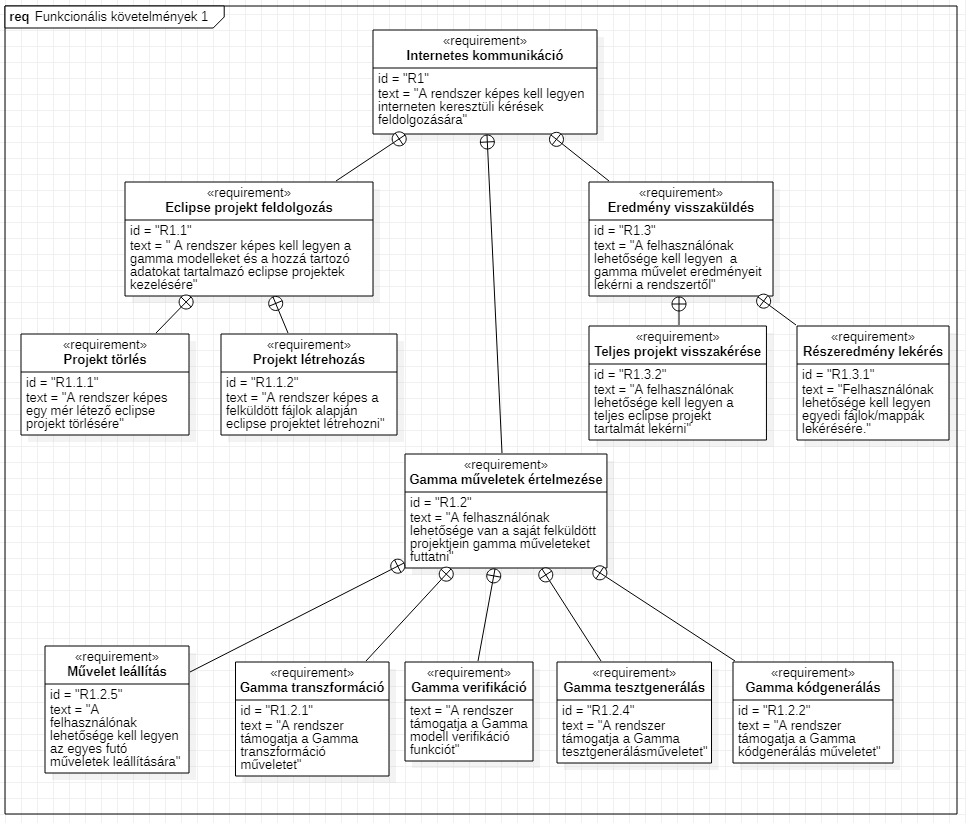
\includegraphics[width=170mm, keepaspectratio]{figures/requierments_placeholder.png}
	\caption{Követelmény hierarchia 1}
	\label{fig:requierments_placeholder}
\end{figure}

\begin{figure}[!ht]
	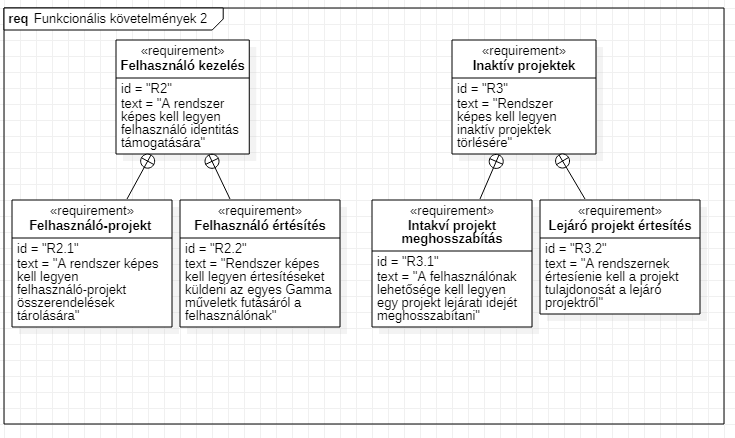
\includegraphics[width=150mm, keepaspectratio]{figures/requierments_2.png}
	\caption{Követelmény hierarchia 2}
	\label{fig:requierements_2}
\end{figure}

A további nem funkcionális követelményeket négy kategóriába soroljuk:
\begin{itemize}
	\item \textbf{Megbízhatóság:} Egy projekten nem futtathatunk két különböző Gamma művelet halmazt
	\item \textbf{Biztonság:} Minden felhasználó csak a saját projektjeit szerkesztheti / saját projektjein futtathat gamma művelet halmazokat / A rendszer képes kell legyen kiszűrni az egyes rosszindulatú felhasználók által megadott fájl elérési utakat / 
	\item \textbf{Teljesítmény:} A rendszer képes kell legyen különböző projekteken ugyanabban az időben Gamma műveletek futtatására. / A rendszer skálázható kell legyen. / A rendszernek nem szabad fölösleges adatot tárolnia. / A rendszer muszáj töröljön minden olyan adatot, amely neki vagy a felhasználó számára nem releváns. / A rendszer képes kell legyen asszinkron módban működni.
	\item \textbf{Felhasználhatóság:} A rendszer megfelelő, HTTP szabvány által előírt válaszokat adni az egyes kérésekre. / A rendszer beszédes értesítéseket kell küldjön a projekt tulajdonosának az egyes Gamma műveletek futási állapotáról.
\end{itemize}

A fentebb leírt követelmények alapján bizonyos technológiai döntéseket kellet hozni a projekt iniciális fázisaiban. Ahhoz, hogy az alkalmazásunk interneten keresztül is elérhető legyen egy webszervert kellet kialakítanunk, ez lesz a rendszer belépési pontja. A webszerver a REST API modern architektúra stílus szabályait betartva lett kialakítva. Mindez a \textit{R1.*} követelmény teljesítése teszi szükségessé. 

Ahhoz, hogy az \textit{R1.2.*} követelmény teljesüljön, a Gamma keretrendszert egy \textit{headless Eclipse}-be kellet becsomagolni. Ezzel megtudjuk oldani azt a problémát, hogy a Gamma az Eclipse IDE-hez van kötve, az így becsomagolt keretrendszert parancssoron keresztül lehet elérni.

Az \textit{R2.*} követelményt eclipse munkaterek (workspace) használatával teljesítjük. A rendszerünk biztosít munkatér létrehozás funkciót a felhasználói oldalon álló kliens szoftvernek, ehhez rendel egy egyedi azonosítót amit visszaküld a kliensnek és mostantól, ezzel az azonosító megadásával tud a kliens további funkciókat elérni. Mindezzel azt érjük el, hogy majdnem semmilyen információt nem kell tárolni a felhasználóról, ezt a feladatot rábízzuk a kliens szoftverre.

Összefoglalva a követelményeket és a technológiai döntéseket, olyan rendszert tervezünk, amely a Gamma keretrendszert elérhetővé teszi a világ számára, oly módon, hogy közben több felhasználói rendszerlogikát támogat az adatok tárolásán és funkciók elérésén. Továbbá, olyan mellék funkciókat is biztosítania kell, mint inaktív projektek automatizált törlése vagy felhasználók értesítése.

A rendszerben érdekelt személyek listája (\textbf{stakeholders}), azaz olyan aktorok, akik valamilyen módon kapcsolatba léphetnek a rendszerrel:
\begin{itemize}
	\item Komplex modellekkel foglalkozó \textbf{mérnökök} (NASA)
	\item \textbf{Egyetemi kutatók}
	\item Olyan \textbf{fejlesztő} aki integrálni akarja a rendszerünket egy harmadik párti alkalmazásba (MagicDraw)
	\item \textbf{Gamma fejlesztő} ,aki erőforrás igényes funkciót akar tesztelni
	\item \textbf{Üzemeltető}, aki a rendszer komponenseit frissíteni tudja
	\item \textbf{Üzleti oldalú kolléga}, aki a rendszert mint szolgáltatás hirdeti/eladja
\end{itemize}

A rendszer jelen formájában nem tartalmazza a fentebb többször említett kliens komponenst, így precíz használati eseteket nehéz definiálni. Ennek ellenére a rendszert teljes funkcionalitását lehet használni, tesztelni valamilyen API tesztelő szoftverrel, mint például PostMan. Olyan kéréseket tudunk küldeni az alkalmazás felé, amelyek teljes körűen szimulálják egy kliens szoftver viselkedését.

Az alapvető elérhető funkciók közé tartozik: a munkatér létrehozás, amely egy felhasználónak dedikált eclipse munkateret hoz létre, amin belül majd további műveleteket lehet végezni; eclipse projekt importálása archivált forrásból egy létező munkatérbe; az importált projektben szereplő, műveleteket leíró fájlok alapján gamma műveletek futtatása; a gamma műveletek által generált elemek visszakérése archivált fájlként; importált eclipse projekt törlése.


%----------------------------------------------------------------------------
\section{Architektúra}
%----------------------------------------------------------------------------
